\documentclass[10pt,twocolumn]{article}
%\documentclass[10pt]{article}
\usepackage{fullpage}
\usepackage{graphicx}

\title{Reducing Write Traffic to Remote Storage}
\author{Ramnatthan Alagappan \and Brandon Davis \and Avinaash Gupta\\\\
Department of Computer Sciences, University of Wisconsin -- Madison}
\begin{document}

\maketitle

\section*{Abstract}
The block device interface enables computer system software such as file
systems to communicate with the storage system. %
When dealing with sector-based storage devices like HDDs, it is necessary to
work with blocks of data. %
But many protocols maintain this block granularity for data in other layers of
the computer system. %
For example, Network Block Device (NBD), iSCSI, and Network File System (NFS)
work with blocks in the network layer, sending entire blocks of data for each
request. %
This can result in excessive data transfer when the useful data in a request is
smaller than the block size. %
With small modifications to NBD to avoid full block requests where possible,
write traffic savings of over 70\% were realized. %

\section{Introduction}
\label{sec:introduction}
Sector-based devices such as HDD can perform operations only on a discrete
segment of data, called a sector. %
A common sector size is 512 bytes. %
Any read/write request to the device should be for a multiple of the
sector size. %

To support and enforce this behavior, Linux provides block special devices. %
In contrast to character special devices, which accept requests for some number
of bytes, block special devices accept requests for some multiple of the sector
size. %
A block device driver transfers data in a BIO (block I/O) struct which requires
that data be maintained at the granularity of one or more sectors. %

In the case of user applications running on a host OS, when a user is writing to
a file, the following occurs: %
\begin{enumerate}
  \item{User issues a \texttt{write} call (by byte)}
  \item{File system receives the request (by byte)}
  \item{File system modifies the appropriate block and optionally
        keeps it in a cache (by block)}
  \item{File system sends a request with BIO struct(s) to the device (by block)}
  \item{Device finalizes the request to the storage system through the transport
    layer (by block)}
\end{enumerate}
The data is maintained at block granularity only at the lowest levels, closest
to the storage system itself. %
Thus a single-byte write will incur a \mbox{\texttt{(blocksize-1)}} byte
overhead only between the file system and the disk. %

When working with remote storage, however, the same overhead can creep into many
layers of the computer system. %
For example, one can look at Network Block Device (NBD) \cite{lopez00}. %
NBD provides a virtual block device on a client machine, which allows access to
the real block device being exported from the server machine. %
Figure~\ref{fig:nbd-system} depicts the pieces of the computer and storage
systems involved when writing to files as before, but this time to remote
storage exported by NBD. %

\begin{figure}[htbp]
  \centering
  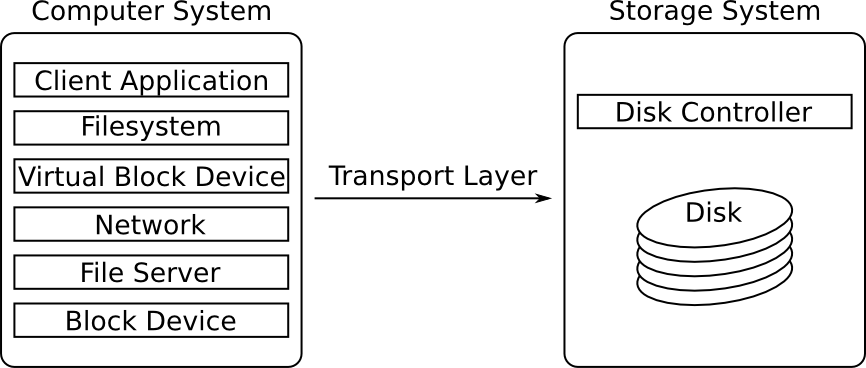
\includegraphics[width=0.50\textwidth]{figs/nbd-system.png}
  \caption{System layers involved when using NBD}
  \label{fig:nbd-system}
\end{figure}

As before, the application need not work with blocks of data. It can write just
a few bytes to a file. %
Also as before, the file system works with data at block granularity. %
This time, however, the data is maintained as blocks through the virtual device,
over the network, and finally to the block device and storage system on the
server. %
The \mbox{\texttt{(blocksize-1)}} byte overhead for a single-byte write is seen through
all of these layers. %

We modified NBD to avoid its strict adherence to block granularity of data
at the network layer. %
In Section~\ref{sec:design}, we describe our technique for avoiding sending blocks
of data in NBD. %
Section~\ref{sec:evaluation} contains an evaluation of the effectiveness of the
technique. %
We discuss the results with regard to similar techniques and limitations of our
implementation in Section~\ref{sec:discussion}. %
Section~\ref{sec:related} gives an overview of related work. %
Future work is outlined in Section~\ref{sec:future}. %
Section~\ref{sec:conclusions} concludes the paper. %

\section{Design and Implementation}
\label{sec:design}


We modified the NBD kernel module (client) from Linux kernel version 3.2.52,
and the server from NBD 3.3 userland source. %
In all, we added approximately 315 lines of code (240 to the client and 75 to
the server). %
We added a file system block cache to the client using the Linux implementation
of radix tree cache. %
A block is cached whenever it is successfully read from or written to the
exported file system. %
On a write request, if a cached copy exists for every logical block being
written, we attempt to send only the pieces of the block that have changed. %

To find these pieces, we logically partition each block into ``chunks'' of equal
size. %
For each block, a bitmap is created with one bit per chunk of the block. %
Chunks that are modified by the write are identified by \texttt{memcmp}. %
If a chunk is found to be modified, the corresponding bit in the bitmap is set 
and that chunk is marked. %
Finally the block's bitmap is sent to the server followed by all marked chunks. %

The server must reconstruct the write data using the bitmap and chunks. %
It reads the original block from the storage device and then writes the chunks 
to their correct positions in the block using the bitmap. %
Finally the server writes the modified block back to the storage device. %

\begin{table} [htbp]
  \centering
  \begin{tabular}{|c|c||c|}
    \hline
    Chunk Size & Bitmap Size & For Savings \\ \hline
    4096 & 1   & 1   \\ \hline
    2048 & 1   & 1   \\ \hline
    1024 & 1   & 1   \\ \hline
    512  & 1   & 1   \\ \hline
    256  & 2   & 1   \\ \hline
    128  & 4   & 1   \\ \hline
    64   & 8   & 1   \\ \hline
    32   & 16  & 1   \\ \hline
    16   & 32  & 3   \\ \hline
    8    & 64  & 9   \\ \hline
    4    & 128 & 33  \\ \hline
    2    & 256 & 129 \\ \hline
    1    & 512 & 513 \\ \hline
  \end{tabular}
  \caption{Chunk sizes and corresponding bitmap sizes. The number of unmodified
    chunks which must be in a block to achieve savings is given in the third
    column.}
  \label{tab:chunksforsavings}
\end{table}

By not sending unmodified chunks of blocks, we can reduce write traffic over the
network. %
The chosen chunk size and corresponding bitmap size will influence the
effectiveness of our technique. %

Table~\ref{tab:chunksforsavings} shows how many unmodified chunks would need to be
found in a block to reduce the transfer size. %
While a chunk size of 1 byte gives us the finest granularity for finding
unmodified chunks, we would need to find 513 of these chunks to actually see a
benefit. %
Conversely, while unmodified chunks of 32 bytes are less common, we only need to
find 1 chunk of this size to benefit from our technique. %

Because the cache in our implementation is intended to be a perfect working 
knowledge of what is on the actual storage device at any given time, we first
ran the experiments with no limit on cache size. %
I.e., no cache eviction is used and all blocks seen by the client are cached. %
For comparison, we also wrote a version with a limited cache size and Least
Recently Used (LRU) replacement policy. %
The performance of each approach is shown in Section~\ref{sub:macro}. %

\section{Evaluation}
\label{sec:evaluation}

We now evaluate our prototype implementation of diff and cache described in
Section~\ref{sec:design}. %
All experiments were run on a virtual machine running Debian Linux (kernel version
3.2.52). %
The machine was given 4GB RAM, and runs on the underlying Intel i7-4700 2.4GHz
processor. %
We evaluate our work in two axes: (i) bytes sent per block with varying sync
probabilities and write sizes and (ii) bytes sent per block using varying chunk
sizes. %

\subsection{Micro-benchmarks}

We evaluate the first case with synthetic microbenchmarks. %
In these benchmarks, we repeatedly write data to a single file being exported by
NBD. %
The chunk size used for microbenchmarks was kept constant at 64 bytes. %
For these experiments, our cache is primed by first reading the entire file
which we will be writing to. %
The parameters to the microbenchmarks are the following:

\begin{itemize}
  \item Sequential vs Random -- Sequential pattern writes to the file as in a log.
  Each write begins where the last write ended. Random pattern randomly seeks to
  any offset in the file before each write.
  \item Write Size -- Size of each write in bytes.
  \item Sync Probability -- Probability for each write that \texttt{fsync} will be
  called following the write.
\end{itemize}

Figure~\ref{fig:randwrite} shows the average bytes sent per block for random
writes with varying write size and sync probability. %
At low sync probabilities, the file system is free to coalesce the writes and so
the average bytes sent per block is higher. %
As the sync probability increases the file system has to flush the writes and
hence result in less modified chunks per block being sent over the network. %
With 4096 byte writes, it is very rare that the writes align with block
boundaries. %
Because we perform our data transformation per logical block, we turn two full
block transfers into two transfers which average to about half of one block. %
This can be seen as the line for 4096 byte write size settles around 2048 bytes
sent per block. %
The baseline shows that a full block will be sent in all cases. %

\begin{figure}[t]
  \centering
  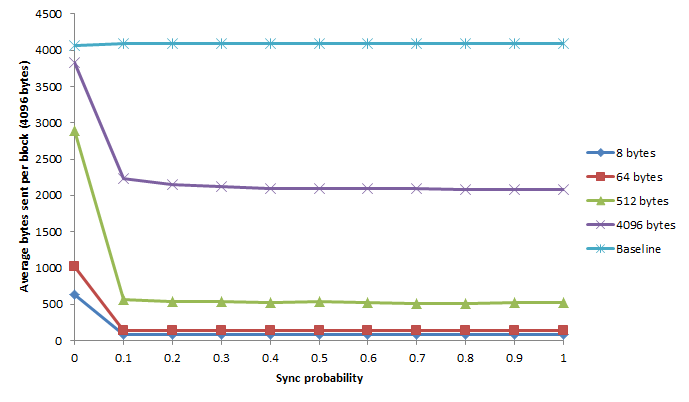
\includegraphics[width=0.50\textwidth]{figs/RandWrite.png}
  \caption{Average bytes sent per block for random writes with varying write sizes and sync 
  probabilities}
  \label{fig:randwrite}
\end{figure}

Figure~\ref{fig:seqwrite} shows a similar graph for sequential writes. %
As mentioned earlier, at low sync probabilities, the file system is free to
coalesce the writes and so the average bytes sent per block is higher. %
As the sync probability increases and reaches 1, we just have to send only the
exact write sized chunk over the network (Note that 512 bytes line converges to
nearly 512 bytes when sync probability is 1). %
We observe some savings even when the write size is 4096 bytes because of
updates to metadata that is smaller than the block containing the metadata. %
The baseline NBD will not be able to achieve this as it has to send the whole
metadata block. %
These savings differ from the savings for 4096 byte writes in the random
workload because none of the sequential writes will span across block
boundaries. %

\begin{figure}[t]
  \centering
  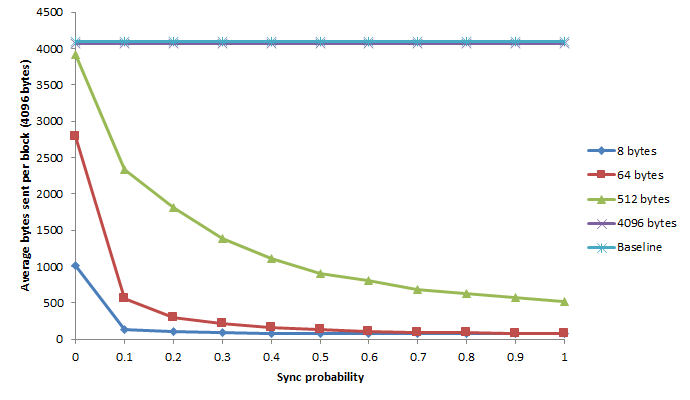
\includegraphics[width=0.50\textwidth]{figs/SeqWrite.png}
  \caption{Average bytes sent per block for sequential writes with varying write sizes and sync 
  probabilities}
  \label{fig:seqwrite}
\end{figure}

\begin{figure}[b]
  \centering
  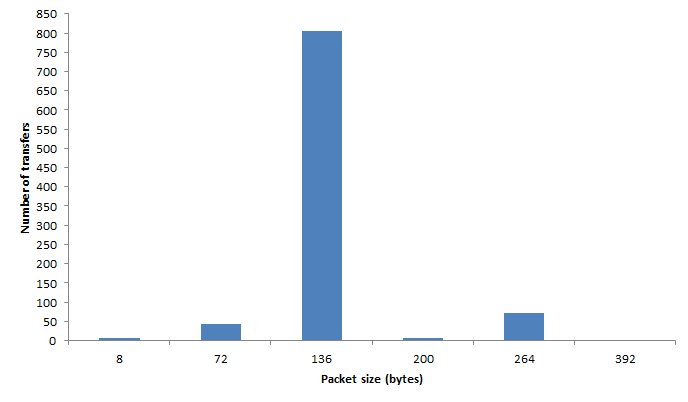
\includegraphics[width=0.50\textwidth]{figs/RandDist.png}
  \caption{Distribution of transfer sizes with 64 bytes chunk size and 64 bytes write size - Random}
  \label{fig:randdist}
\end{figure}

\begin{figure}[t]
  \centering
  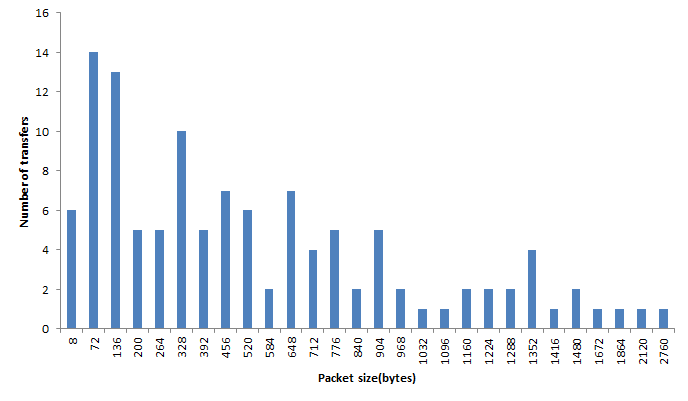
\includegraphics[width=0.50\textwidth]{figs/SeqDist.png}
  \caption{Distribution of transfer sizes with 64 bytes chunk size and 64 bytes write size - Sequential}
  \label{fig:seqdist}
\end{figure}

Figure~\ref{fig:randdist} and Figure~\ref{fig:seqdist} show the distribution of
transfer sizes for a fixed write size of 64 bytes and sync probability of 0.1. %
We can observe that the distribution is dense near small transfer sizes and is
sparser for large transfer sizes. %

\subsection{Macro-benchmark}
\label{sub:macro}

We evaluate various chunk size in our implementation with SysBench MySQL OLTP
macrobenchmark \cite{kopytoc04}. %
We varied the chunk size in our implementation from 1 byte to 4096 bytes. %
For these workloads, we began with an empty cache, in contrast to the primed
cache we used in our microbenchmark analysis. %
The results are shown in Figure~\ref{fig:oltp}. %

With very small chunk sizes like 1 byte and 2 bytes, we incur constant bitmap
overhead of 512 and 256 bytes respectively, which contributes substantially to
the transfer size. %
As the chunk size increases, the bitmap overhead is reduced but the opportunity
to locate unmodified chunks decreases. %

Our experiments show that for this OLTP workload, the optimum value of chunk
size is between 8 and 32 bytes. %
At 16 byte chunk size, we see a reduction of 73\% to the average bytes sent per
block. %
At the largest chunk size (4096 bytes), the bitmap overhead is minimized but the
entire block will be sent even if one byte has changed. %
Interestingly, we observe a small amount of savings even with the largest chunk
size. %
Occasionally, writes to a block do not actually change the content of that
block. %
Baseline NBD would send the entire block anyway, but our technique will identify
that there is no difference in the block and will avoid that transfer. %

The above experiment was performed with a cache that can hold the entire working
set of the benchmark. %
We also evaluate the average bytes sent per block with a more traditional cache. %
The OLTP macro benchmark originally required around 4000 cache entries without
eviction, so we limited the cache size to 256 entries which is about 6\% of the
original requirement. %
To handle the large working set, we employed an LRU replacement policy for our
cache. %

Figure~\ref{fig:withcacheevic} shows the average bytes sent per block
with the limited cache and eviction policy. %
We note that the limited cache size and cache eviction does not eliminate all
benefits of our technique. %
There is a moderate increase in average transfer size as we are forced to send
an entire block when we have no entry for it in our cache. %

\begin{figure}[htbp]
  \centering
  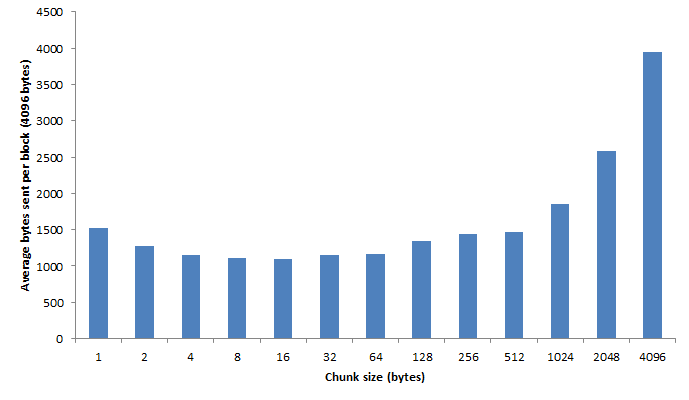
\includegraphics[width=0.50\textwidth]{figs/OLTP.png}
  \caption{Average bytes sent per block with varying chunk sizes}
  \label{fig:oltp}
\end{figure}

\begin{figure}[htbp]
  \centering
  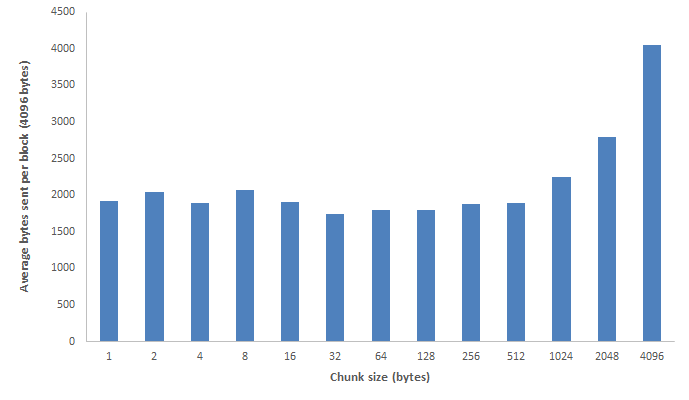
\includegraphics[width=0.50\textwidth]{figs/WithCacheEvic.png}
  \caption{Average bytes sent per block with varying chunk sizes with LRU cache}
  \label{fig:withcacheevic}
\end{figure}

\section{Discussion}
\label{sec:discussion}
%In this section, we discuss two things. 1. How our method compares against
%block level compression techniques. 2. How our technique performs in Copy-On-Write
%file systems like BTRFS.

\subsection {Lossless Block Compression}
We studied how compression techniques work with block data. %
We used ZLIB library \cite{gailly04} (which internally uses the DEFLATE
compression algorithm) to compress all the file blocks in regular files in user
home directories. %
With highest compression level enabled, the average compression ratio per block
was 0.325. %
The lowest level of compression yielded a compression ratio of 0.345. %
Block level compression techniques have to be lossless since the blocks have to be
reconstructed exactly. %
But our technique is in a way lossy compression since we can use the contents
present on the NBD server (which is an external knowledge from the compression)
to reconstruct the exact data. %
Experimental studies show that the maximum compression ratio that can be
achieved with block compression is around ???. %
Table~\ref{table:comptechniques} shows the compression ratios and percentage
savings for home directories of 2 different users. %


\begin{table}[ht]
  \centering 
  \begin{tabular}{|c|c|c|} % centered columns (4 columns)
    \hline
    User & High & Low \\ \hline
    User1 & 72.70 & 70.55  \\
    User2 & 62.62 & 60.48  \\ \hline
  \end{tabular}
  \caption{Percentage savings using compression techniques} 
  \label{table:comptechniques} 
\end{table}

In our best case, where nothing has been changed as part of a write, we achieve
a compression ratio very close to 0 and our savings is close to 100 percent.
This is not feasible with lossless block compression because there is a
constant overhead of compression metadata even when there is no change to the
contents.

\subsection{BTRFS}
Next, we studied how our technique performs with COW file systems. We ran our
experiments with NBD server exposing the remote storage as BTRFS file system
\cite{rodeh12}. %
Since COW file systems do not update content of block in-place, we expected to
see little improvement using our technique of caching by logical block. As
expected, we observed that our technique does not work well with BTRFS. This
experiment was run with a large cache and no eviction was required. 

Figure~\ref{fig:btrfsseqwrite} shows that there are still some savings, though
not as dramatic as with ext2. %
We believe that this is due to in-place updates of the superblock in BTRFS.

\begin{figure}[htbp]
  \centering
  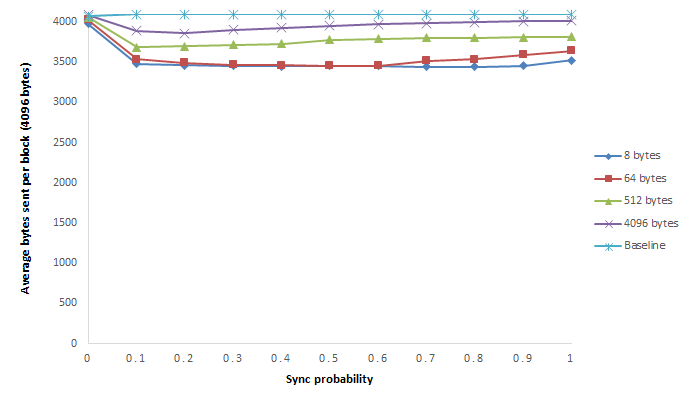
\includegraphics[width=0.50\textwidth]{figs/BTRFSSeqWrite.png}
  \caption{BTRFS - Sequential Writes - Average bytes sent per block with varying write sizes and sync probability}
  \label{fig:btrfsseqwrite}
\end{figure}

Figure~\ref{fig:btrfsseqdist} confirms that most of the written blocks are not
found in the cache due to BTRFS' COW behavior. %
A completely modified block found in the cache results in transfer size of 4104
bytes, but we see mainly transfers of 4096 bytes. %
This is the case when we cannot perform a diff and just send the data as usual. %

\begin{figure}[htbp]
  \centering
  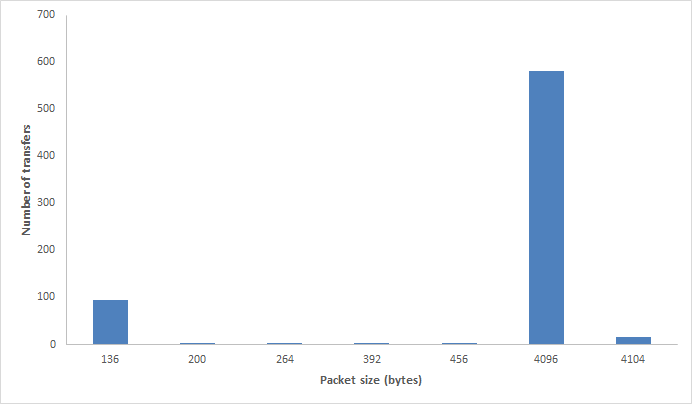
\includegraphics[width=0.50\textwidth]{figs/BTRFSSeqDist.png}
  \caption{BTRFS - Sequential Writes -Distribution of transfer sizes with 64 bytes chunk size and 64 bytes write size}
  \label{fig:btrfsseqdist}
\end{figure}

  
\section{Related Work}
\label{sec:related}

Active Disks \cite{acharya98, riedel97, boboila12} utilize computing
resources within the storage system to perform useful work. %
This can include processing data before writing to the device or after reading
from it. %
It can also include filtering data to avoid transferring unwanted data back to
the caller. %
In our technique, the NBD server is a user level process. %
However, to implement our technique in a protocol such as iSCSI \cite{satran04}, the
storage system would need to be active. %

Bjorling promotes the transition away from block device interfaces for new
storage devices such as SSD\cite{bjorling13}. %
Bjorling argues that the block device interface is not expressive enough to
leverage performance opportunities in state of the art devices. %
The Object Storage model \cite{factor05} is one approach to storage without
blocks. %
Instead of a flat array of homogeneous blocks, the object store exports storage
as a collection of objects. %
Allocation decisions are made only at the device layer, and thus there is no
abstraction akin to blocks which creeps into other areas of the computer system. %

\section{Future Work}
\label{sec:future}
Amazon Elastic Block Storage \cite{amazon} provides persistent block level
storage for applications running in Amazon EC2. %
We would like to examine how block level transfers happen in this setup, and how
applications typically use Amazon EBS service. %
There are many questions to be answered about proprietary remote block device
services. %
``Can multiple clients connect to the same block device?'' %
``If so, how can we ensure that all clients see consistent data?'' %
``How do SCSI reservations work in this model?'' %

Our findings also lead to the question of where the block device interface
belongs. %
Perhaps a file system could be designed which is divided into block-independent
and block-dependent layers. %
The block-dependent layer could be placed as close as possible to the storage
system, thus removing the block constraint from upper layers. %
In the case of non-HDD storage, the block-dependent layer could even be disabled
in favor of software that better utilizes the specific features of the storage
device, e.g. parallel banks, Copy on Write, etc. %

\section{Conclusions}
\label{sec:conclusions}

Adhering to specific interfaces in generic domains can be detrimental in some
cases. %
We have shown that network transfers of blocks using the block interface is one
such example. %
With minor modifications to how different layers can work with most appropriate
interfaces, we have shown that substantial savings are possible. %
Specifically, by breaking the block interface requirements in the network layer
of the system, we have shown a savings of 70\% in network traffic for some
workloads. %
Our findings join the ranks of byte-addressable phase change memory, SSDs with
characteristics unseen in HDDs, and differentiated storage services, all giving
reasons to take a closer look at the block interface. %

\begin{thebibliography}{9}

\bibitem{acharya98}
  Anurag Acharya, Mustafa Uysal, Joel Saltz,
  \emph{Active disks: programming model, algorithms and evaluation},
  ACM SIGPLAN Notices,
  v.33 n.11,
  p.81-91,
  Nov. 1998.

\bibitem{riedel97}
  Riedel, E. and Gibson, G.,
  \emph{Active Disks - Remote Execution for Network-Attached Storage},
  Technical Report CMU-CS-97-198,
  December 1997.

\bibitem{boboila12}
  S. Boboila, Y. Kim, S. S. Vazhkudai, P. Desnoyers, and G. M. Shipman,
  \emph{Active Flash: Out-of-core Data Analytics on Flash Storage},
  In MSST,
  2012.

\bibitem{factor05}
  M. Factor, K. Meth, D. Naor, O. Rodeh, and J. Satran.,
  \emph{Object Storage: the future building block for storage systems},
  In LGDI ’05: Proceedings of the 2005 IEEE International Symposium on Mass Storage Systems and Technology,
  pp. 119–123, 
  Washington, DC, USA,
  2005. 

\bibitem{bjorling13}
  Matias Bjorling, Philippe Bonnet, Luc Bouganim, Niv Dayan, et al.,
  \emph{The necessary death of the block device interface},
  In 6th Biennial Conference on Innovative Data Systems Research (CIDR),
  2013.

\bibitem{kopytoc04}
  Alexey Kopytov,\\
  \mbox{\emph{SysBench: a system performance benchmark}},
  http://sysbench.sourceforge.net/index.html,
  2004.

\bibitem{sandberg85}
  Sandberg, R., Goldberg, D., Kleiman, S., Walsh, D., and Lyon, B.,
  \emph{Design and Implementation of the Sun Network Filesystem},
  Proceedings of the Summer 1985 USENIX Conference,
  Portland OR,
  pp. 119-130,
  June 1985.

\bibitem{rodeh12}
  Rodeh, Ohad, Josef Bacik, and Chris Mason,
  \emph{Brtfs: The linux b-tree filesystem},
  IBM Research Report RJ10501 (ALM1207-004),
  2012.

\bibitem{satran04}
  Satran, Julian, and Kalman Meth,
  \emph{Internet small computer systems interface (iSCSI)},
  2004.

\bibitem{lopez00}
  Lopez, Marin, and P. T. A. Arturo Garcia Ares,
  \emph{The network block device},
  Linux Journal 2000.73es,
  2000.

\bibitem{amazon}
  Amazon.com, Inc.,
  \emph{Amazon Elastic Block Store (EBS)},
  http://aws.amazon.com/ebs/.

\bibitem{gailly04}
  Gailly, Jean-loup, and Mark Adler,
  \emph{Zlib compression library},
  2004.

\end{thebibliography}

\end{document}
